%ROUNDING WHOLE NUMBERS - WORKSHEET 0 (IN-CLASS INSTRUCTION)
\documentclass[12pt, letterpaper, fleqn]{article}

% ----------------------------------------------------------
% PACKAGES
% ----------------------------------------------------------
\usepackage{graphicx}
\usepackage{xcolor}
\usepackage[most]{tcolorbox}
\usepackage{amsmath, amssymb}
\usepackage{fancyhdr}
\usepackage[utf8]{inputenc}
\usepackage[T1]{fontenc}
\usepackage{enumitem}
\usepackage{geometry}
\usepackage{tikz}
\usepackage{needspace}
\usepackage{multicol}

\usetikzlibrary{arrows.meta, calc, shapes.geometric}

% ----------------------------------------------------------
% PAGE SETUP
% ----------------------------------------------------------
\usepackage{times}
\geometry{letterpaper, top=1.25in, bottom=1.25in, marginpar=0.5in}

% ----------------------------------------------------------
% HEADER / FOOTER
% ----------------------------------------------------------
\newcommand{\logowidth}{3cm}
\setlength{\headheight}{20pt}
\setlength{\footskip}{40pt}

\pagestyle{fancy}
\fancyhf{}
\fancyhead[C]{\small\bfseries Rounding Whole Numbers}
\fancyfoot[L]{\raisebox{2pt}{
\includegraphics[width=\logowidth]{../kss.png}}}
\fancyfoot[C]{\thepage}
\fancyfoot[R]{3.11.0}

\renewcommand{\footrulewidth}{0.2pt}

% ----------------------------------------------------------
% THEME COLOR
% ----------------------------------------------------------
\definecolor{customteal}{HTML}{2fbdb9}

% ----------------------------------------------------------
% HELPER MACROS
% ----------------------------------------------------------
\newcommand{\blank}{\underline{\hspace{2.2cm}}}
\newcommand{\blanklong}{\underline{\hspace{6.5cm}}}
\newcommand{\blankshorter}{\underline{\hspace{1.5cm}}}

% ----------------------------------------------------------
% DOCUMENT
% ----------------------------------------------------------
\begin{document}

\textbf{Name:} \underline{\hspace{5cm}}
\hfill
\textbf{Date:} \underline{\hspace{3cm}}\\

\begin{tcolorbox}[colback=customteal!20]
    \large\textcolor{black}{\textbf{Rounding Whole Numbers}}
\end{tcolorbox}

\vspace{3mm}
\noindent
Rounding makes numbers simpler to use.
\begin{itemize}
    \item When rounding to the nearest **10**, look at the **ones** place. If it is 5 or more, round up!
    \item When rounding to the nearest **100**, look at the **tens** place.
\end{itemize}

\vspace{3mm}
\begin{center}
\begin{tikzpicture}[scale=0.8]
\draw[thick] (0,0) -- (10,0);
\draw[thick] (0,0.2) -- (0,-0.2) node[below] {30};
\draw[thick] (5,0.2) -- (5,-0.2) node[below] {35 (Midpoint)};
\draw[thick] (10,0.2) -- (10,-0.2) node[below] {40};
\filldraw[red] (3,0) circle(0.15) node[above] {33};
\filldraw[green] (7,0) circle(0.15) node[above] {37};
\end{tikzpicture}
\end{center}
* 33 is closer to 30. It rounds down to 30.
* 37 is closer to 40. It rounds up to 40.

\newpage
\begin{tcolorbox}[colback=customteal!20]
    \large\textcolor{black}{\textbf{Guided Practice}}
\end{tcolorbox}

\vspace{5mm}
\begin{enumerate}[itemsep=2.5cm, leftmargin=0.6cm]
\item Round to the nearest 10:
  \begin{itemize}[itemsep=0.8cm]
    \item 42 $\rightarrow$ \blank
    \item 85 $\rightarrow$ \blank
    \item 78 $\rightarrow$ \blank
  \end{itemize}

\item Round to the nearest 100:
  \begin{itemize}[itemsep=0.8cm]
    \item 130 $\rightarrow$ \blank
    \item 475 $\rightarrow$ \blank
    \item 850 $\rightarrow$ \blank
  \end{itemize}
\end{enumerate}

\end{document}
